\documentclass{university}

\course{هوش مصنوعی}
\subject{تمرین سوم بخش اول}
\professor{دکتر رهبان}

\begin{document}

\setupdocument

\section{}
برای سادگی دامنه متغییرها را 
\lr{$\{k, c, z\}$}
که اول کلمات خروج، چاه و زندان است در نظر می‌گیریم.

\subsection{}
\subsubsection{قیدهای \lr{Binary}}
اگر رو میزان باد بین دو در متوالی
\lr{$i$}
و
\lr{$j$}
حالت‌بندی کنیم، داریم:
\begin{itemize}
    \item کم: \lr{$(X_i,X_j) \in \{(k,z), (z,k)\}$}
    \item زیاد: \lr{$(X_i,X_j) \in \{(k,c), (c,k), (c,c), (c,z), (z,c)\}$}
    \item بدون باد: \lr{$(X_i,X_j) \in \{(z,z)\}$}
\end{itemize}

\subsubsection{قیدهای \lr{Unary}}
اگر رو میزان باد دو سمت در 
\lr{$i$} 
حالت‌بندی کنیم، داریم:
\begin{itemize}
    \item کم و کم: \lr{$X_i \in \{k, z\}$}
    \item کم و زیاد: \lr{$X_i \in \{k, z\}$}
    \item کم و بدون باد: \lr{$X_i \in \{z\}$}
    \item زیاد و زیاد: \lr{$X_i \in \{k, c, z\}$}
    \item زیاد و بدون باد: \lr{$X_i \in \{z\}$}
    \item بدون باد و بدون باد: \lr{$X_i \in \{z\}$}
\end{itemize}

\subsection{}
ابتدا قیدهای یونری را اعمال می‌کنیم. اگر در 6 را خروج در نظر بگیریم، طبق 
\lr{constraint}
دوم باینری، در 1 باید چاه باشد. در ادامه بین در 1 و 2، 
\lr{constraint}
اول باینری برقرار نمی‌شود. پس همینجا متوجه می‌شویم که نمی‌توانیم به متغیر 
\lr{$X_1$}
مقدار تخصیص دهیم. پس متغیر 
\lr{$X_6$}
نباید مقدار خروج داشته باشد.

\begin{gather*}
    X_6 = k \\
    \text{\lr{apply unary constraints:}} \\
    X_1 \in \{k, z\} \\
    X_2 \in \{k, z\} \\
    X_3 \in \{k, z\} \\
    X_4 \in \{k, c, z\} \\
    X_5 \in \{k, c, z\} \\
    \text{\lr{forward checking:}} \\
    X_1 \in \{\} \\
    X_2 \in \{k, z\} \\
    X_3 \in \{k, z\} \\
    X_4 \in \{k, c, z\} \\
    X_5 \in \{c\} \\
\end{gather*}

\subsection{}
متغییری با کمترین تعداد مقادیر مجاز باید مقداردهی شود. پس در این حالت یک از متغییرهای 
\lr{$X_4$} 
یا 
\lr{$X_6$}
که هر دو یک مقدار مجاز دارند باید مقداردهی شود.

\subsection{}
متغییر 
\lr{$X_5$}
را ثابت در نظر می‌گیریم سپس با توجه به 
\lr{Constaint}ها
مقادیر مجاز بقیه متغییرها را تعیین می‌کنیم.
\begin{gather*}
    X_5 = z \\
    X_1 = \{k, z\} \\
    X_2 = \{k, z\} \\
    X_3 = \{k, z\} \\
    X_4 = c \\
    X_6 = c
\end{gather*}
راه‌حل های ممکن در جدول 
\ref{table:solution}
آمده است.

\begin{table}[htbp]
    \centering
    \begin{tabular}{|c|c|c|c|c|c|c|}
        \hline
        \# & \lr{$X_1$} & \lr{$X_2$} & \lr{$X_3$} & \lr{$X_4$} & \lr{$X_5$} & \lr{$X_6$} \\
        \hline
        \hline
        1 & \lr{$k$} & \lr{$z$} & \lr{$k$} & \lr{$c$} & \lr{$z$} & \lr{$c$} \\
        \hline
        2 & \lr{$z$} & \lr{$k$} & \lr{$z$} & \lr{$c$} & \lr{$z$} & \lr{$c$} \\
        \hline
    \end{tabular}
    \caption{راه‌حل های ممکن با فرض به زندان منتهی شدن در پنجم}
    \label{table:solution}
\end{table}

\subsection{}
برای حل این مسئله، همه قیدها را تعریف می‌کنیم.

تابع 
\lr{$w(D_i)$}
را میزان بادی که از زیر در برای در منتهی به سرنوشت 
\lr{$D_i$}
می‌آید تعریف می‌کنیم. سپس روی 
\lr{$D_i$}
که 
\lr{$1 \leq i \leq d$}
است، مانند قسمت الف و به صورت زیر حالت بندی می‌کنیم. 

\begin{gather*}
    w(D_i) : (X_j,X_k) \in \{(D_j,D_k)|max(w(D_j), w(D_k))<= w(D_i)\}
\end{gather*}

قیدهای باینری به صورت بالا بدست می‌ایند.
حال به سراغ قیدهای یونری می‌رویم.
برای هر زوج مرتب 
\lr{$(D_i,D_j)$}
که 
\lr{$1 \leq i,j \leq d$}
است، حالت‌بندی می‌کنیم.
\begin{gather*}
    (w(D_i), w(D_j)) : X_k \in \{D_k|D_k \leq min(w(D_i), w(D_j))\}
\end{gather*}

با توجه به قیود، گراف قیود مانند شکل 
\ref{fig:constraintGraph}
می‌شود. حال اگر نود مشخص شده با رنگ قرمز را حذف کنیم، گراف ما یک درخت بدون دور می‌شود. طبق قضیه مطرح شده در کلاس، می‌دانیم این 
\lr{CSP}
در زمان 
\lr{$O((n-1) \times d^2)$}
قابل حل است. این زمان نسبت به 
\lr{$n$}
خطی است. حال مسئله را 3 بار جدا حل می‌کنیم. هر بار مقدار 
\lr{$X_n$}
که از گراف حذف شده بود، را یکی از مقادیر دامنه 
(\lr{$\{k, c, z\}$})
قرار می‌دهیم. با این کار کل مسئله در زمان 
\lr{$O(d \times (n-1) \times d^2) = O(n \times d^3)$}
قابل حل است که شرایط خطی بودن نسبت به تعداد متغیرها را براورده می‌کند.

\begin{figure}[htbp]
    \centering
    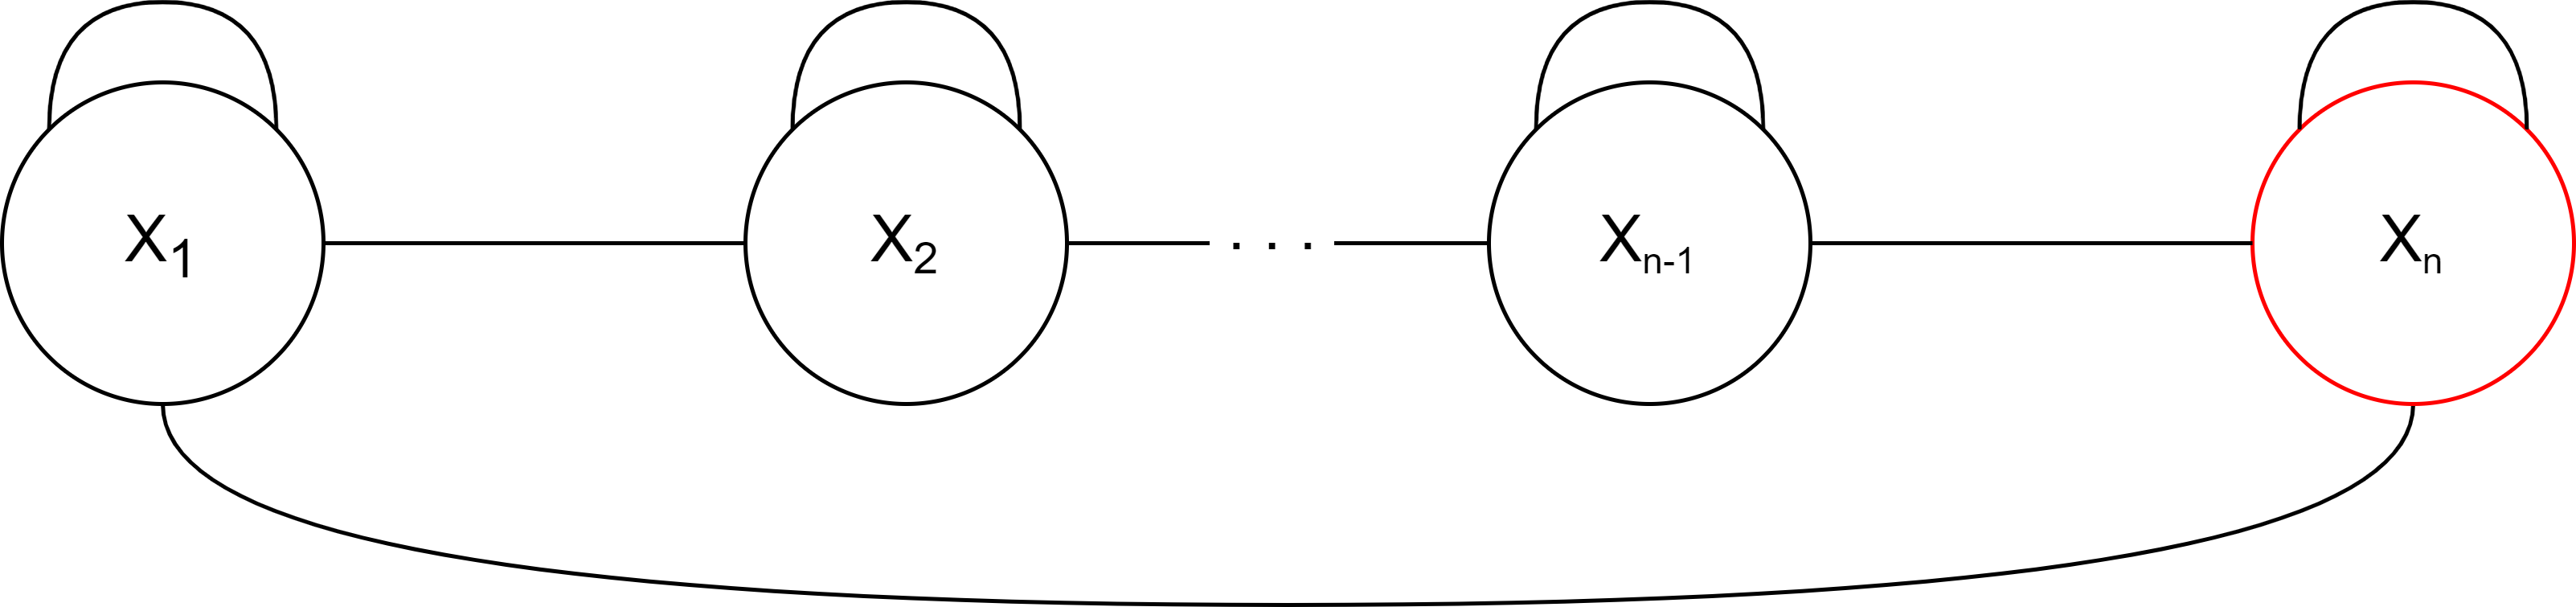
\includegraphics[width=0.8\textwidth]{assets/constraint-graph.drawio.png}
    \caption{گراف قیود}
    \label{fig:constraintGraph}
\end{figure}

\subsection{}
اگر از جستجوی 
\lr{backtracking}
استفاده کنیم، 
\lr{$\text{branching factor} = d$}
و 
\lr{$\text{depth} = n$}
است. پس درخت جستجو دارای 
\lr{$d^n$}
برگ است. پس در بدترین حالت که آخرین برگ جواب مسئله است، 
\lr{$d^n-1$}
بازگشت داشته‌ایم. 

\end{document}